%%
%% Copyright Guy Taylor 2012
%%
%%
\chapter{Background}

\section{Background}
Initial trials at the University of Edinburgh established that breathing movements and respiratory
frequencies could be measured accurately and reproducibly using accelerometers attached to the
chest of human subjects (including hospital patients), reaching levels of 96\% accuracy\cite{BatesLingMannArvind2010}.
It was therefore decided to produce a custom piece of hardware dedicated
to this task that might be suitable for longer-term clinical use. The accelerometer device used in the
trial was a prototype based on the Orient-3 wireless sensor platform originally designed for use in
real-time motion capture. For the trial however, the monitoring system did not use the wireless
transceiver but instead used off-line analysis.
With the aim to reach medical trials, a smaller and lower-powered device was designed to allow
longer-term monitoring for further investigations of accelerometer-based respiratory monitoring on
patients The new hardware was named the Respire and is a significant improvement over the
prototype device. The Respire integrates four key components of the prototyped Orient-2/3 onto a
single more accessible device to allow further development and testing:- a \ac{MCU},
accelerometer, radio and flash memory. However, the original Orient-3 firmware was incompatible
with the Respire and therefore a new firmware needed to be designed and implemented, with an
emphasis on reducing the power requirements of the system.

\section{Power Management}
To calculate the power needed to run a device you first need to measure the power use during
active use \(P_(active)\), power use during sleeping \(P_(sleep)\) and the percentage of time in a state of
activity \(Duty\).
\[
  P_(average) = D x P_(active) + (1-D) x P_(sleep)
\]
\[
  P_(active) >> P_(sleep)
\]
It is most common however that \(P_(active)\) and \(P_(sleep)\) are fixed or only small reductions can be
made. It is therefore most effective in normal applications to reduce the duty, this reduction is most
assisted by faster wake up periods.


\begin{wrapfigure}{l}{0.5\textwidth}
  \vspace{-10pt}
  \begin{center}
    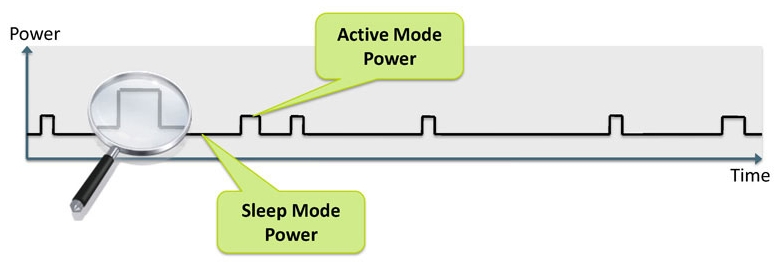
\includegraphics[width=0.4\textwidth, keepaspectratio=true]{images/lowenergysystemsoverview_croped.jpg}
  \end{center}
  \caption[Sleep Graph]{Sleep Graph \cite{EFM32Tech}}
  \vspace{-10pt}
\end{wrapfigure}

In any small wireless devices the main power consumer is the radio during use, therefore it is key to
minimise its duty cycle. Mediation devices exist between the edge nodes and the core of a network,
allowing data to be buffered and processed away from the edge. This mediation allows the edge
devices to "sleep" more predictably and with greater duration and depth, decreasing the edge
power needs\cite{Sapio & Tsouri, 2010, Edgar2003}. % TODO


This system of moving the power towards the centre of the network is more effective in hierarchical networks
where there is a clear distinction, \eg by a larger battery, between the nodes
and the mediation devices. This allows the mediation device to be awake for
longer without the battery expectancy of the global networks decreasing.

\section{Respire Device Components}

\subsection{Energy Micro EFM32 \ac{MCU}}

\begin{wrapfigure}{r}{0.8\textwidth}
  \vspace{-10pt}
  \begin{center}
    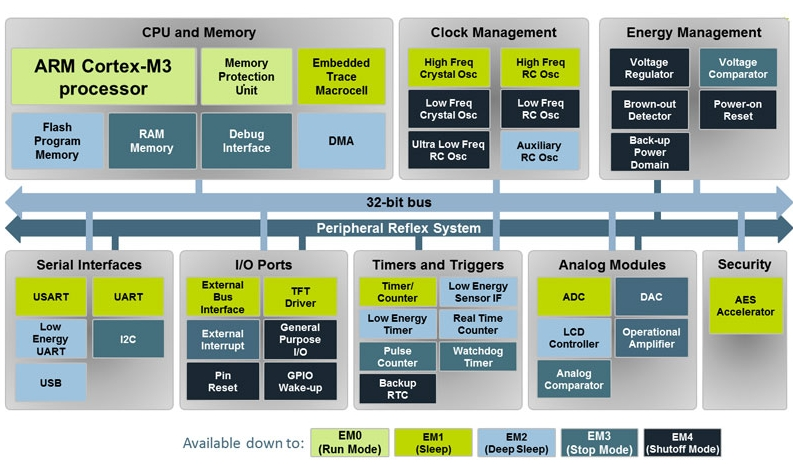
\includegraphics[width=0.7\textwidth, keepaspectratio=true]{images/efm32_block_croped.jpg}
  \end{center}
  \caption[EFM32 Block Diagram]{EFM32 Block Diagram \cite{EFM32Tech}}
  \vspace{-10pt}
\end{wrapfigure}

The Energy Micro EFM32 series of \ac{MCU} is a system-on-a-chip designed from the bottom
up for low energy applications. At the core of the EFM32 is an ARM Cortex-M3 \ac{MCU} enabling the
power and flexibility to reduce energy needs by decreasing duty time and closely interacting with its
peripherals. In the same silicon to the \ac{MCU} is an array of specially designed low-power modules,
many of them, that are independently wired together allowing \ac{MCU} free communication and
interaction enhanced by a \ac{DMA} controller.

\subsection{ARM Cortex-M3}
The ARM Cortex-M3 is a 32-bit Harvard style, \ac{RISC} \ac{MCU}. It is designed
around the ARMv7 instruction set with the addition of Thumb
and Thumb-2 compressed instruction sets. The Cortex-M is the sub series dedicated to low power
system-on-a-chip \acp{MCU}, with the Cortex-M3 being specifically for realtime applications.


The Cortex-M3 series was designed to both provide good performance with low power but also
decrease the complexity of programming, the normally complex 8 and 16-bit architectures. This
reduction in complexity is mainly achieved by the use of assembly free interrupts and the full
standardisation of configurations through the use of memory mapped registers. This standardisation
allows the many implementations of Cortex-M3, with different system-on-a-chip peripherals, to be
easily learnt. The assembly free interrupts allow all code to be viewed in a single language and thus
preventing hidden or obscured processes. This ease of implementation is assisted by a full debugging
subsystem, with optional in-circuit emulator, accessible via a new 2 to 3 pin interface reducing the
size on the device and thus allowing debugging be kept in the production layout. This new debugging
interface, \ac{SWD}, has a built in ability to directly communicate back to the
debugger using the optimal 3rd, \ac{SWO}, pin. With the \ac{SWO} the programmer can use
standard consoles printing techniques without disruption of the program flow.


The Thumb reduced instruction set is a 16-bit wide subset of the main ARM set that allows multiple
instructions to be compressed into a single instruction read, thus reducing \ac{I/O} latency. The Thumb-2
instruction set extend thumb set by the utilising 32-bit instructions and thus provide more
functionality and packing, thus providing a 30\% improvement. This combination lowers the speed to
power ratio and also the program memory needed. This performance is also achieved with the
simple, false always, branch speculation within the three stage pipeline.


The Cortex-M3's most important improvements are the new interrupt system and single bit
manipulation system. The new interrupt system reduces interrupt latency, allows direct wake from
sleep and also allows chaining, with priority. chaining of interrupts significantly reducing interrupt
latency in instances where interrupts are likely to happen simultaneously. The priority system allows
key events to be reordered reducing the chance of delay, producing a more deterministic system. A
new bit manipulation system allows individual bits to be changed without reading, modifying and
writing the whole byte, reducing IO. The "bit-banding" is also combined with the previous
generation unaligned memory system allowing single bit, byte, half word and the full 32-bit word to
be uniquely addressed.


Throughout all ARM architecture there is the CIMIS standardisation.....

\cite{Sadasivan 2006} \cite{Arm2012, EnergyMicro2011}


\subsection{\acf{PRS}}

\begin{wrapfigure}{l}{0.5\textwidth}
  \vspace{-10pt}
  \begin{center}
    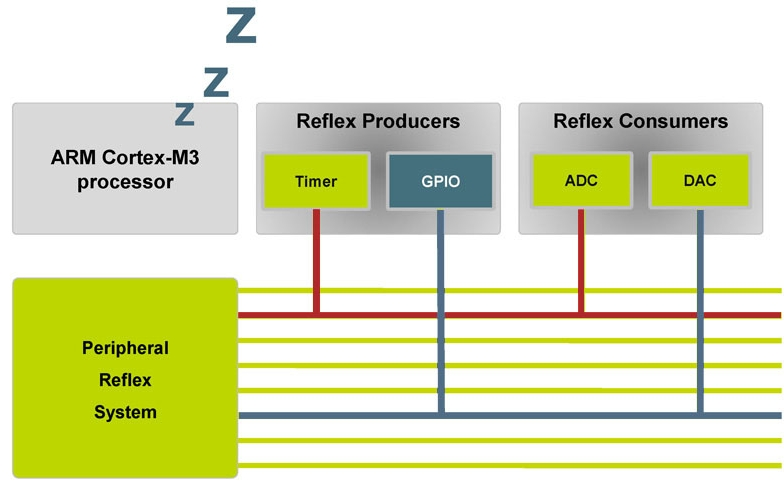
\includegraphics[width=0.4\textwidth, keepaspectratio=true]{images/peripheralreflexsystem_croped.jpg}
  \end{center}
  \caption[EFM32 \ac{PRS} Diagram]{EFM32 \ac{PRS} Diagram \cite{EFM32Tech}}
  \vspace{-10pt}
\end{wrapfigure}

The \ac{PRS} is a technology that allows the peripherals in the system-on-a-
chip, external to the \ac{MCU}, to independently interact and thus not force the \ac{MCU} to wake from
sleep. To enable such control, the system has predefined production and consumption interfaces on
each module, these range from automated ADC every second triggered by the \ac{RTC} to using receipt
of \ac{USART} data to trigger switching of a device pin. Many of these peripherals clock independently of
the \ac{MCU} so this system can even work in the deepest sleep states.

\subsection{\acf{CMU} and \acf{EMU}}

\begin{wrapfigure}{r}{0.4\textwidth}
  \vspace{-10pt}
  \begin{center}
    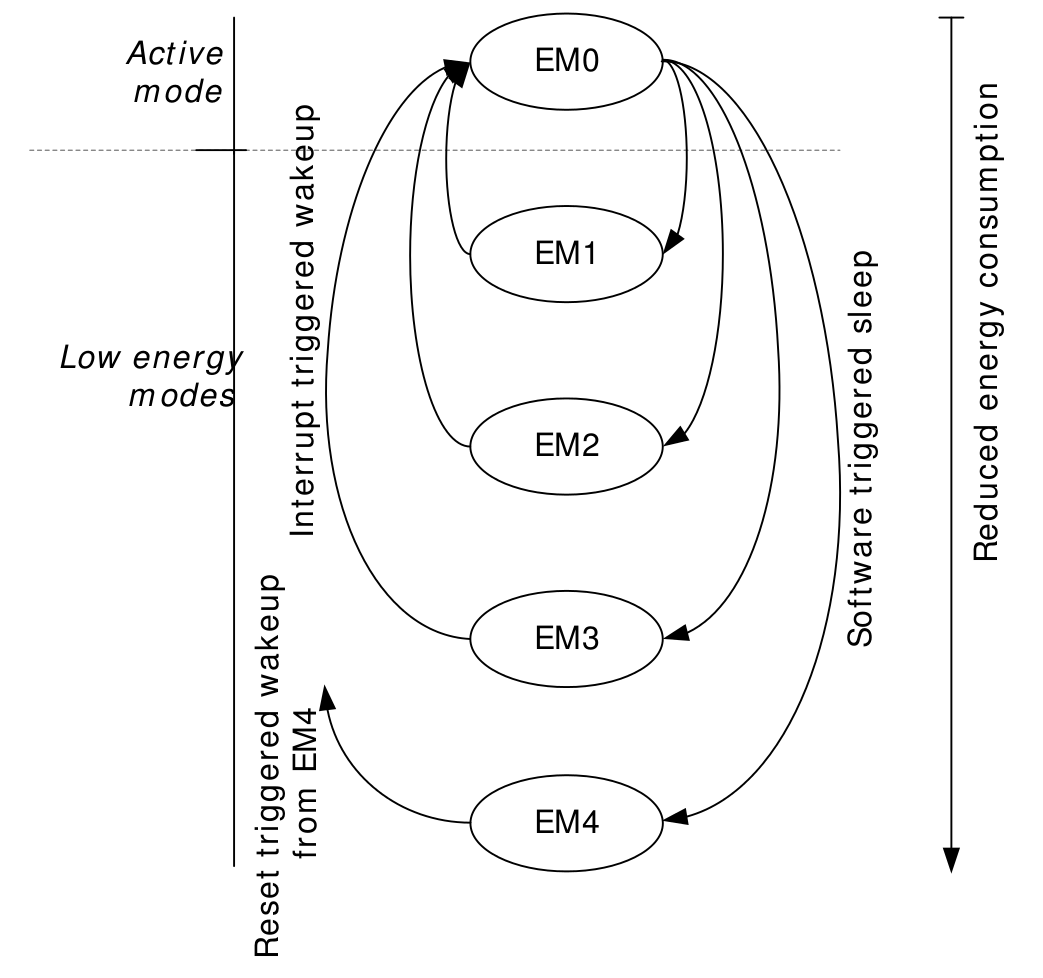
\includegraphics[width=0.3\textwidth, keepaspectratio=true]{images/efm32_sleep_states.png}
  \end{center}
  \caption[EFM32 \ac{EMU} Diagram]{EFM32 \ac{EMU} Diagram \cite{EFM32Ref}}
  \vspace{-10pt}
\end{wrapfigure}

The EFM32s ground up approach of designing all models in the system, except from the \ac{MCU} and \ac{DMA} controller,
allows a powerful clock and energy management system that allows individual clocking and enabling
of each subsystem allowing modules to consume no power when not in use. The clock management
system also enables several clock to be chosen for each module, allowing the programmer is most
effectively choose the set of clocks needed. Thank you management system also extend directly into
the \ac{MCU}, allowing extra sleep states to be added to the Cortex-M3. These extra sleep states allow
the \ac{MCU} to gradually decrease the number of high frequency clocks the maintain state and
also includes full hibernation of the chip with only the externally clocked subsystems
enabled. From these sleep states EFM32 has a fast wake-up time allowing shorter burst
periods and deeper sleeps.

\subsection{Nordic nRF24L01+}
The Nordic nRF24L01+ (hereafter referred to as NRF24) is a low-power digital radio
designed to work in the 2.4Ghz ISM radio bands. The radio enables fast 2Mbit transfer
between devices but only supports half duplex communications and therefore cannot transmit and
receive data simultaneously.

\subsection{MMA8451Q Accelerometer}
This component was included to support the high-accuracy measurements needed to monitor
breathing movements in a small, low-energy package.

\subsection{Flash Memory}
A 64-Mbit flash memory chip is included in the Respire to facilitate offline storage of sensor data
when no network is available.


